\documentclass[aps,prl,reprint,superscriptaddress,nofootinbib]{revtex4-2}
\usepackage[T1]{fontenc}
\usepackage{amsmath,amssymb,amsthm,bm,mathtools}
\usepackage{graphicx,booktabs,microtype}
\usepackage{tikz}
\usetikzlibrary{arrows.meta,positioning,calc,decorations.pathreplacing}
\usepackage[hidelinks]{hyperref}
\newcommand{\repolink}{\href{https://github.com/SamMausberg/returning-constructor}{\nolinkurl{github.com/SamMausberg/returning-constructor}}}
\usepackage[nameinlink,noabbrev]{cleveref}
\newtheorem{theorem}{Theorem}
\usepackage{aliascnt}
\newaliascnt{lemma}{theorem}
\newtheorem{lemma}[lemma]{Lemma}
\aliascntresetthe{lemma}
\newaliascnt{proposition}{theorem}
\newtheorem{proposition}[proposition]{Proposition}
\aliascntresetthe{proposition}
\newaliascnt{corollary}{theorem}
\newtheorem{corollary}[corollary]{Corollary}
\aliascntresetthe{corollary}
\crefname{lemma}{Lemma}{Lemmas}
\Crefname{lemma}{Lemma}{Lemmas}
\crefname{proposition}{Proposition}{Propositions}
\Crefname{proposition}{Proposition}{Propositions}
\crefname{corollary}{Corollary}{Corollaries}
\Crefname{corollary}{Corollary}{Corollaries}
% APS style capitalizes numbered references mid-sentence.
\crefname{theorem}{Theorem}{Theorems}
\crefname{table}{Table}{Tables}
\theoremstyle{definition}\newtheorem{definition}[theorem]{Definition}
\newcommand{\Tr}{\operatorname{Tr}}
\newcommand{\id}{\operatorname{id}}
\newcommand{\rank}{\operatorname{rank}}
\newcommand{\supp}{\operatorname{supp}}
\newcommand{\norm}[1]{\left\lVert#1\right\rVert}
\newcommand{\ket}[1]{|#1\rangle}
\newcommand{\bra}[1]{\langle#1|}
\newcommand{\SW}{\mathsf S}
\newcommand{\ha}{h_2}
\newcommand{\Pone}{\mathcal P_1}
\newcommand{\positive}[1]{\left[#1\right]_+}
\DeclareMathOperator{\Bin}{Bin}
\setlength{\emergencystretch}{1em}
\newcommand{\statement}[1]{\input{statements/#1.tex}}

\usepackage{capt-of}
\hypersetup{pdftitle={Comment on Emergence of constructor-based irreversibility in quantum systems},pdfauthor={Samuel Mausberg}}
\begin{document}
\title{Comment on ``Emergence of constructor-based irreversibility in quantum systems: Theory and experiment''}
\author{Samuel Mausberg}
\affiliation{Independent researcher}
\email{samuelmausberg@gmail.com}
\date{October 2, 2026}
\maketitle

\noindent\begin{minipage}{\columnwidth}
\centering
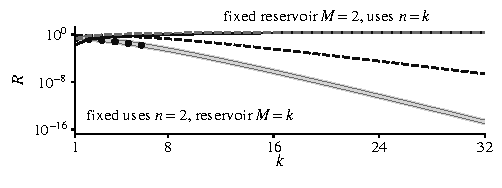
\includegraphics[width=\columnwidth]{figures/comment_ratio.pdf}
\captionof{figure}{Current-output infidelity divided by reservoir fidelity at $\eta=\pi/4$, with $p=\ket0\bra0$ and $\tau=I/2$: solid, $p\to\tau$; dashed, $\tau\to p$. The upper pair tends to $2$; the falling pair tends to zero. Rational channel updates and certified spectral intervals give the curves and markers. The gray band encloses the forward falling ratio using $e\le R\le4e$, with certified current infidelity $e$.}
\label{c:fig}
\end{minipage}\par\medskip

We examine the repeated homogenizer of Ref.~\cite{prl} with all correlations retained. The current-error limits agree in both directions; the published capability infimum fails separately.

The definitions changed between versions. Preprint v1~\cite{prlv1}, p.~2, uses a supremum and a two-variable limit; its p.~3 limits take uses first. Published Eqs.~(3)--(7), (12)--(13)~\cite{prl} instead use an infimum, a fixed first-use numerator, and uses before accuracy. The supplement, Eqs.~(9)--(10), substitutes the designated initializer and assumes $S(n)\approx S(1)^n$. Reference~\cite{vm}, Eqs.~(8)--(13), uses current infidelity; its preprint leaves the joint limit unspecified, while the published Eq.~(11) and the thesis~\cite{thesis}, Eq.~(5.4), take reservoir size first.

Let $U_\eta=\cos\eta I+i\sin\eta\,\SW$, $0<\eta\le\pi/2$, with inputs $a$ and $M$ cells initially in $b^{\otimes M}$. Write $\rho_{M,n}$ for output $n$, $\Omega_{M,n}$ for the joint outputs, and $\sigma_{M,n}$ for the reservoir. A fresh $b$ ancilla sweeping $k$ cells defines $\Phi_{b,k}$. Disjoint-gate exchange~\cite{gp} gives
\begin{equation}
 \Omega_{M,n}=\Phi_{b,n}^{M}(a^{\otimes n}),\quad
 \sigma_{M,n}=\Phi_{a,M}^{n}(b^{\otimes M}).
 \label{c:exchange}
\end{equation}
Every finite block relaxes to its boundary product state. For a pure boundary, its channel is triangular in excitation sectors, with diagonal moduli $\cos^{r+t}\eta$ and only the vacuum peripheral. Full swap shifts the block. For a mixed boundary, an all-pure-eigenstate branch of a sufficiently long channel power gives strict contraction.

Use squared Uhlmann fidelity, $0<f=F(a,b)<1$, and $R_{M,n}=[1-F(\rho_{M,n},b)]/F(\sigma_{M,n},b^{\otimes M})$. Comparing with the invariant grid $b^{\otimes(n+M)}$ gives reservoir fidelity at least $f^n$. Relaxation therefore yields
\begin{equation}
 \lim_{M\to\infty}R_{M,n}=0,\qquad
 \lim_{n\to\infty}R_{M,n}=(1-f)f^{-M}.
 \label{c:limits}
\end{equation}
Thus $\lim_n\lim_M R=0$ and $\lim_M\lim_n R=+\infty$; diagonal sequences exclude a joint limit. Fidelity symmetry gives identical limits for the transpose task (Fig.~\ref{c:fig}).



For the published infimum, set $p=\ket0\bra0$, $\tau=I/2$, $q=\cos^2\eta\in(0,1)$, $M\ge2$, and $e_M=(1-\sqrt{1-q^{2M}})/2$. With first-output channel $\mathcal O_p$, the definitions are
\begin{align}
 V_e&=\{\omega:F(\mathcal O_p(\omega),\tau)\ge1-e\},\nonumber\\
 S_e(n)&=\inf_{\omega\in V_e}F(\omega,\Phi_{p,M}^{n}(\omega)).
\end{align}
For $q\ge1/3$, choose $\omega=\ket1\bra1\otimes\tau^{\otimes(M-1)}$. Its first-output Bloch coordinate is $(2q-1)q^{M-1}$, whose magnitude is at most $q^M$, so $\omega\in V_{e_M}$. For $q<1/3$, keep the first cell in $\ket1$, give the second coordinate $z_2=q(1-2q)/(1-q)\in[0,1]$, and put the rest in $\tau$. The second update $z\mapsto qz+(1-q)z_2$, starting at $z=2q-1$, gives zero: the first output is exactly $\tau$.

Both product initializers are orthogonal to the attractor $p^{\otimes M}$. Hence $S_{e_M}(n)\to0$ and $e_M/S_{e_M}(n)\to+\infty$, contradicting the published forward uses-first conclusion at every strict partial swap. A surviving asymmetry under whole-memory return is analyzed in Ref.~\cite{companion}.

\begin{acknowledgments}
The author selected the research questions and is responsible for the content. GPT-6 Astra (OpenAI) assisted with derivations, source comparison, and writing, and Claude (Anthropic) was used for review and editing.
\end{acknowledgments}
\noindent{\raggedright\textit{Data availability.} Exact plotting data and code are available at \repolink{}.\par}

\begin{thebibliography}{6}
\bibitem{prl} C. Marletto et al., Phys. Rev. Lett. \textbf{128}, 080401 (2022), arXiv:2009.14649v2; Supplemental Material, Eqs.~(9)--(10).
\bibitem{prlv1} C. Marletto et al., arXiv:2009.14649v1, pp.~2--3.
\bibitem{vm} M. Violaris and C. Marletto, New J. Phys. \textbf{24}, 113030 (2022), arXiv:2205.11310v1.
\bibitem{thesis} M. Violaris, arXiv:2505.22834v1, Chap.~5.
\bibitem{gp} V. Giovannetti and G. M. Palma, Phys. Rev. Lett. \textbf{108}, 040401 (2012), arXiv:1105.4506, Eqs.~(4)--(7).
\bibitem{companion} {\raggedright S. Mausberg, Memory return in quantum machines (2026), \repolink{}.\par}
\end{thebibliography}
\end{document}
